\graphicspath{{./figures/}}
\title{rust / sandboxing 1}
\date{}
\begin{document}
\begin{frame}
    \titlepage
\end{frame}

\begin{frame}{last time}
    \begin{itemize}
    \item static analysis possibilities
        \begin{itemize}
        \item very practical analyses: finding common mistake patterns
        \item more ambitious/inaccurate: safety properties like no UAF/out-of-bounds
        \end{itemize}
    \item information flow analysis / static or dynamic
        \begin{itemize}
        \item does data move from source to sink
        \item e.g. does private info (keypresses, phone numbers, etc.) leak?
        \item e.g. can attacker control SQL statement, shell command?
        \item e.g. where does malware's network input end up on filesystem?
        \end{itemize}
    \item toward better programming languages
        \begin{itemize}
        \item what about C/C++ makes people use it
        \item idea of escape hatches for limits of safe languages
        \end{itemize}
    \end{itemize}
\end{frame}

\section{logistics note}
\begin{frame}{logistics note}
    \begin{itemize}
    \item FUZZ deadline
    \item quiz
    \end{itemize}
\end{frame}

\subsection{general syntax}
\usetikzlibrary{positioning,shapes.callouts}
\begin{frame}[fragile,label=rustHelloWorld1]{simple Rust syntax (1a)}
\begin{minted}{Rust}
fn main() {
    println!("Hello, World!\n");
}
\end{minted}
\end{frame}

\begin{frame}[fragile,label=rustHelloWorld1]{simple Rust syntax (1b)}
\begin{minted}{Rust}
fn main() {
    let name = "World";
    println!("Hello, {}!\n", name);
}
\end{minted}
\end{frame}

\begin{frame}[fragile,label=rustHelloWorld2]{simple Rust syntax (2)}
\begin{minted}[fontsize=\fontsize{11}{12}]{Rust}
fn timesTwo(number: i32) -> i32 {
    return number * 2;
}

/* or last value automatically returned: */
fn timesTwo(number: i32) -> i32 {
    number * 2
}
\end{minted}
\end{frame}

\begin{frame}[fragile,label=rustHelloWorld3]{simple Rust syntax (3)}
    \begin{minted}[fontsize=\fontsize{11}{12}]{Rust}
struct Student {
    name: String,
    id: i32,
}

fn get_example_student() -> Student {
    Student {
        name: String::from("Example Fakelastname"),
        id: 42,
    }
}
\end{minted}
\end{frame}

\begin{frame}[fragile,label=rustHelloWorld4]{simple Rust syntax (4)}
    \begin{minted}[fontsize=\fontsize{10}{11}\selectfont,escapeinside=||]{Rust}
fn factorial(number: i32) -> i32 {
    let mut|\tikzmark{mut}| result = 1;
    let mut index = 1;
    while index <= number {
        result *= index;
        index = index + 1;
    }
    return result;
}
\end{minted}
    \begin{tikzpicture}[overlay,remember picture]
        \coordinate (box) at (current page.center);
        \begin{visibleenv}<2>
            \node[my callout=mut,anchor=center,align=left] at ([yshift=2cm]box) {
                ``result'' is a mutable variable \\
                type automatically inferred as i32 (32-bit int)
            };
        \end{visibleenv}
    \end{tikzpicture}
\end{frame}



\subsection{references}
\subsubsection{basic example}
\begin{frame}[fragile,label=rustTimesTwoB]{Rust references}
\vspace{-.25cm}
    \begin{minted}[fontsize=\fontsize{10}{11}\selectfont,escapeinside=||]{Rust}
fn main() {
    let mut x: u32 = 42;

    {
        let y: &mut u32 = &mut x;
        *y = 100;
    }

    let z: &u32 = &x;

    println!("x = {}; z = {}", x, z);
}
\end{minted}
\end{frame}




\subsubsection{in context}

\usetikzlibrary{positioning,shapes.callouts}
\begin{frame}[fragile,label=rustTimesTwo]{Rust example with refs}
    \begin{minted}[fontsize=\fontsize{10}{11}\selectfont,escapeinside=||]{Rust}
use std::io;

fn main() {
    println!("Enter a number: ");

    let mut|\tikzmark{mut}| input = String::new();
    // could have also written:
    //   let mut input: String = String::new();
    
    io::stdin().read_line(&mut|\tikzmark{ref}| input);

    // parse number or fail with an error message
    let number: u32|\tikzmark{int}| = input.trim().parse()
        .expect("That was not a number!");
    println!("Twice that number is: {}", number * 2);
}
\end{minted}
    \begin{tikzpicture}[overlay,remember picture]
        \coordinate (box) at (current page.center);
        \begin{visibleenv}<2>
            \node[my callout=mut,anchor=center,align=left] at ([yshift=2cm]box) {
                ``input'' is a mutable variable \\
                type is automatically inferred as String
            };
        \end{visibleenv}
        \begin{visibleenv}<3>
            \node[my callout=ref,anchor=center,align=left] at ([yshift=-2cm]box) {
                pass mutable reference to input
            };
        \end{visibleenv}
        \begin{visibleenv}<4>
            \node[my callout=int,anchor=center,align=left] at (box) {
                number is an immutable unsigned 32-bit integer
            };
        \end{visibleenv}
    \end{tikzpicture}
\end{frame}




\subsection{basic ownership}
\begin{frame}{rules to stop dangling pointers (1)}
    \begin{itemize}
    \item objects have an single \myemph{owner}
    \item owner is the only one allowed to modify an object
    \item owner can give away ownership
    \item simplest version: only owner can access object
    \item never have multiple references to object --- always move/copy
    \end{itemize}
\end{frame}

\begin{frame}[fragile,label=rustOwnership1]{Rust objects and ownership (1a)}
    \begin{minted}[fontsize=\fontsize{9}{10}\selectfont]{Rust}
fn mysum(vector: Vec<u32>) -> u32 {
    let mut total: u32 = 0;
    for value in &vector {
        total += value
    }
    return total
}

fn foo() {
    let vector: Vec<u32> = vec![1, 2, 3];
    let sum = mysum(vector);
    // **moves** vector into mysum()
         // philosophy: no implicit expensive copies
    
    println!("Sum is {}", sum);
    // ERROR
    println!("vector[0] is {}" , vector[0]);
}
\end{minted}
    \begin{tikzpicture}[overlay,remember picture]
        \begin{visibleenv}<2>
            \node[anchor=center,font=\small,draw=black,ultra thick,fill=white] at (current page.center){
            \begin{lstlisting}[language={},style=script]
   Compiling lecture-demo v0.1.0 (file:///home/cr4bd/spring2017/cs4630/...
error[E0382]: use of moved value: `vector`
  --> src/main.rs:16:34
   |
13 |     let sum = mysum(vector);
   |                     ------ value moved here
...
16 |     println!("vector[0] is {}" , vector[0]);
   |                                  ^^^^^^ value used here after move
\end{lstlisting}
        };
        \end{visibleenv}
    \end{tikzpicture}
\end{frame}

\begin{frame}[fragile,label=rustOwnership2]{Rust objects and ownership (2)}
    \begin{minted}[fontsize=\fontsize{9}{10}\selectfont]{Rust}
fn mysum(vector: Vec<u32>) -> u32 {
    let mut total: u32 = 0
    for value in &vector {
        total += value
    }
    return total
}

fn foo() {
    let vector: Vec<u32> = vec![1, 2, 3];
    let sum = mysum(vector.clone());
    // give away a copy of vector instead
        // mysum will dispose, since it owns it
    
    println!("Sum is {}", sum);
    println!("vector[0] is {}" , newVector[0]);
}
\end{minted}
    \begin{tikzpicture}[overlay,remember picture]
        \begin{visibleenv}<2>
            \node[anchor=center,font=\small,draw=black,ultra thick,fill=white,align=center] at (current page.center){
            mysum borrows a copy
        };
        \end{visibleenv}
    \end{tikzpicture}
\end{frame}

\begin{frame}{moving?}
    \begin{itemize}
    \item moving a Vec --- really copying a pointer to an array and its size
    \item cloning a Vec --- making a copy of the array itself, too
    \vspace{.5cm}
    \item Rust defaults to moving non-trivial types
    \item some trivial types (u32, etc.) are copied by default
    \end{itemize}
\end{frame}

\begin{frame}[fragile,label=rustOwnership3]{Rust objects and ownership (3)}
    \begin{minted}[fontsize=\fontsize{9}{10}\selectfont]{Rust}
fn mysum(vector: Vec<u32>) -> (u32, Vec<u32>) {
    let mut total: u32 = 0
    for value in &vector {
        total += value
    }
    return (total, vector)
}

fn foo() {
    let vector: Vec<u32> = vec![1, 2, 3];
    let (sum, newVector) = mysum(vector);
    // give away vector, get it back
    
    println!("Sum is {}", sum);
    println!("vector[0] is {}" , newVector[0]);
}
\end{minted}
    \begin{tikzpicture}[overlay,remember picture]
        \begin{visibleenv}<2>
        \node[anchor=center,font=\small,draw=black,ultra thick,align=center,fill=white] 
            at (current page.center) {
        mysum ``borrows'' vector, then gives it back \\
        uses pointers
        };
        \end{visibleenv}
    \end{tikzpicture}
\end{frame}

\begin{frame}{ownership rules}
    \begin{itemize}
    \item exactly one owner at a time
    \item giving away ownership means you \myemph{can't use object}
        \begin{itemize}
        \item<2> common idiom --- temporarily give away object
        \end{itemize}
    \item either give object new owner or deallocate
    \end{itemize}
\end{frame}



\subsection{exercise}
\begin{frame}[fragile,label=ownerRulesExer]{ownership exercise}
If called like \texttt{p = foo(p)}, which follow single-owner rule?
\begin{tikzpicture}
\node (left) {
\begin{lstlisting}[language=C,style=smaller]
// (A)
char *foo(char *p) {
    free(p);
    return NULL;
}

// (B)
char *foo(char *p) {
    p = realloc(p, strlen(p) + 100);
    strcat(p, "test");
    return p;
}
\end{lstlisting}
};
\node[anchor=north west] (right) at (left.north east) {
\begin{lstlisting}[language=C,style=smaller]
// (C)
char *global;
char *foo(char *p) {
    if (p) free(p);
    return global;
}

// (D)
char *foo(char *p) {
    p[0] = 'A';
    return p;
}
\end{lstlisting}
};
\end{tikzpicture}
\end{frame}


\section{Rust: stopping dangling pointers}
\begin{frame}<1>[label=dangleRules]{rules to stop dangling pointers (2)}
    \begin{itemize}
    \item objects have an single \textbf{owner}
    \item owner can give away ownership permanently
        \begin{itemize}
        \item object is ``moved''
        \end{itemize}
    \item \myemph<1>{owner can let someone borrow object \myemph<2>{\textbf{temporarily}}}
        \begin{itemize}
        \item must know when object is given back
        \end{itemize}
    \item only \myemph<3>{\textbf{modify}} object when exactly one user
        \begin{itemize}
        \item owner or exclusive borrower
        \end{itemize}
    \end{itemize}
\end{frame}


\subsection{borrowing}

\begin{frame}[fragile,label=rustBorrowing1]{borrowing (1)}
    \begin{minted}[fontsize=\fontsize{10}{11}\selectfont]{Rust}
fn mysum(vector: &Vec<u32>) -> u32 {
    let mut total: u32 = 0
    for value in vector {
        total += value
    }
    return total
}

fn foo() {
    let vector: Vec<u32> = vec![1, 2, 3];
    let sum = mysum(&vector);
    // automates (vector, sum) = mysum(vector) idea
    
    println!("Sum is {}", sum);
    println!("vector[0] is {}" , vector[0]);
}
\end{minted}
\end{frame}

\begin{frame}[fragile,label=dangling1a]{dangling pointers? (1a)}
\begin{lstlisting}[language=C,style=small]
int *dangling_pointer() {
    int array[3] = {1,2,3};
    return &array[0]; // not an error
}
\end{lstlisting}
\hrulefill
    \begin{minted}[fontsize=\small]{Rust}
fn dangling_pointer() -> &mut i32 {
    let array = vec![1,2,3];
    return &mut array[0]; // ERROR
}
\end{minted}
\begin{tikzpicture}[overlay,remember picture]
    \begin{visibleenv}<2>
    \node[fill=white,draw,very thick,font=\scriptsize,align=left] at (current page.center) {
\begin{lstlisting}[language={},style=smaller]
error[E0106]: missing lifetime specifier
  --> src/main.rs:19:25
   |
19 | fn dangling_pointer() -> &mut i32 {
   |                          ^ expected lifetime parameter
   |
   = help: this function's return type contains a borrowed value,
           but there is no value for it to be borrowed from
\end{lstlisting}
};
    \end{visibleenv}
\end{tikzpicture}
\end{frame}

\begin{frame}[fragile,label=dangling1b]{dangling pointers? (1b)}
\begin{minted}[fontsize=\small]{Rust}
/* 'static = "valid forever" */
fn dangling_pointer() -> &'static mut i32 {
    let array = vec![1,2,3];
    return &mut array[0]; // ERROR
}
\end{minted}
\begin{tikzpicture}[overlay,remember picture]
    \begin{visibleenv}<2>
    \node[fill=white,draw,very thick,font=\scriptsize,align=left] at (current page.center) {
\begin{lstlisting}[language={},style=smaller]
error[E0515]: cannot return value referencing local variable `v`
 --> src/lib.rs:3:12
  |
3 |     return &v[0];
  |            ^-^^^
  |            ||
  |            |`v` is borrowed here
  |            returns a value referencing data owned
  |            by the current function
\end{lstlisting}
};
    \end{visibleenv}
\end{tikzpicture}
\end{frame}


\begin{frame}[fragile,label=dangling2]{dangling pointers? (2)}
\begin{lstlisting}[language=C,style=small]
int *ptr;
int dangling_pointer(int *array) {
    ptr = &array[0];
    return array[0];
}
\end{lstlisting}
\hrulefill
    \begin{minted}[fontsize=\small]{Rust}
static mut ptr : &i32 = &0;
fn dangling_pointer(v: Vec<i32>) -> i32 {
    ptr = &v[0];
    return v[0];
}
\end{minted}
\begin{tikzpicture}[overlay,remember picture]
    \begin{visibleenv}<3>
    \node[fill=white,draw,very thick,font=\scriptsize,align=left] at (current page.center) {
\begin{lstlisting}[language={},style=smaller]
error[E0133]: use of mutable static is unsafe
              and requires unsafe block
 --> src/lib.rs:3:5
  |
3 |     ptr = &v[0];
  |     ^^^ use of mutable static
  |
  = note: mutable statics can be mutated by
          multiple threads: aliasing violations
          or data races will cause undefined behavior
\end{lstlisting}
};
    \end{visibleenv}
    \begin{visibleenv}<2>
    \node[fill=white,draw,very thick,font=\scriptsize,align=left] at (current page.center) {
\begin{lstlisting}[language={},style=smaller]
error[E0597]: `v` does not live long enough
 --> src/lib.rs:3:12
  |
2 | fn dangling_pointer(v: Vec<i32>) -> i32 {
  |                     - binding `v` declared here
3 |     ptr = &v[0];
  |     -------^---
  |     |      |
  |     |      borrowed value does not live long enough
  |     assignment requires that `v` is borrowed for `'static`
4 |     return v[0];
5 | }
  | - `v` dropped here while still borrowed
\end{lstlisting}
};
    \end{visibleenv}
\end{tikzpicture}
\end{frame}

\begin{frame}[fragile,label=rustBorrowing2a]{borrowing (2a)}
\begin{minted}[fontsize=\fontsize{10}{11}\selectfont]{Rust}
fn add1(vector: &mut Vec<u32>) {
    for value in vector {
        *value += 1
    }
}

fn foo() {
    let mut vector: Vec<u32> = vec![1, 2, 3];
    add1(&mut vector);
    println!("vector[0] is {}" , vector[0]);
}
\end{minted}
\end{frame}

\begin{frame}[fragile,label=rustBorrowing2b]{borrowing (2b)}
\begin{minted}[fontsize=\fontsize{10}{11}\selectfont]{Rust}
fn add1(vector: &mut Vec<u32>) {
    for value in vector {
        *value += 1
    }
}

fn foo() {
    let mut vector: Vec<u32> = vec![1, 2, 3];
    // what previous example was basically shorthand for
    {
        let borrowed = &mut vector;
        // borrowing vector here...
        add1(borrowed);
        // until here
    }
    println!("vector[0] is {}" , vector[0]);
}
\end{minted}
\end{frame}


\begin{frame}{borrow tracking}
    \begin{itemize}
    \item compiler finds \textit{lifetime} of borrowing
        \begin{itemize}
        \item when is new reference to object created
        \item when is last use of reference to object
        \end{itemize}
    \item compiler checks for overlap with all other borrowings of that object
    \end{itemize}
\end{frame}



\subsection{exercise}
\begin{frame}[fragile,label=noDangleApply1Exer]{applying rules (1)}
\begin{itemize}
\item single owner, someone can borrow temporarily
\item only modify if exactly one user
\end{itemize}
\begin{tikzpicture}
\node (left) {
\begin{lstlisting}[language={},style=script]
let mut x = 42;    // (1)
let p = &mut x;    // (2)
*p = 10;           // (3)
println!("{}", x); // (4)
\end{lstlisting}
};
\node[anchor=north west] (right) at (left.north east) {
\begin{lstlisting}[language=C++,style=script]
int x = 42;        // (1)
int *p = &x;       // (2)
*p = 10;           // (3)
printf("%d\n", x); // (4)
\end{lstlisting};
};
\end{tikzpicture}
\begin{itemize}
\item Exercise 1/2/3/4: The owner of x on line 1/2/3/4 is:
    \begin{itemize}
    \item A. (original owner) the variable x
    \item B. (borrowed) the pointer/reference p
    \end{itemize}
\end{itemize}
\end{frame}

\begin{frame}[fragile,label=noDangleApply2Exer]{applying rules (2)}
\begin{itemize}
\item single owner, someone can borrow temporarily
\item only modify if exactly one user
\end{itemize}
\begin{tikzpicture}
\node (left) {
\begin{lstlisting}[language={},style=script]
let mut x = 42;    // (1)
let p = &mut x;    // (2)
*p = 10;           // (3)
println!("{}", x); // (4)
*p = 11;           // (5)
\end{lstlisting}
};
\node[anchor=north west] (right) at (left.north east){
\begin{lstlisting}[language=C++,style=script]
int x = 42;        // (1)
int *p = &x;       // (2)
*p = 10;           // (3)
printf("%d\n", x); // (4)
*p = 11;           // (5)
\end{lstlisting};
};
\end{tikzpicture}
\begin{itemize}
\item Rust rufuses to compile left-side: x being used while borrowed by p
\item Which changes would avoid this problem?
    \begin{itemize}
    \item A. use \texttt{*p} in the println!
    \item B. make \texttt{p} mutable, reassign \lstinline|p = &mut x| after line (4)
    \item C. take a non-mutable reference to x instead of a mutable one
    \end{itemize}
\end{itemize}
\end{frame}


\subsection{lifetimes}

\subsubsection{motivation}
\begin{frame}[fragile,label=whyLifetime1]{why lifetimes? (1)}
\begin{minted}[fontsize=\fontsize{12}{13}]{Rust}
let x = vec![1, 2, 3, 4];
let mut q = &x[1];
{
    let mut r = &x[1];
    let y = vec![5, 6, 7, 8];
    if random() == 0 {
        r = &y[1]; // SHOULD BE FINE
        q = &y[1]; // SHOULD BE ERROR
    }
    println!("{}", *r);
}
println!("{}", *q);
\end{minted}
\begin{itemize}
\item need to prevent \texttt{q} referring to values that live too long
\end{itemize}
\end{frame}

\begin{frame}[fragile,label=whyLifetime2]{why lifetimes? (2)}
\begin{minted}[fontsize=\fontsize{12}{13}]{Rust}
fn mystery(ptr: &i32, vec: &Vec<i32>) -> &i32 {...}

fn example() {
    ...
    let mut x = vec![1, 2, 3, 4];
    let mut q = &x[1];
    {
        let mut y = vec![5, 6, 7, 8];
        q = mystery(q, &y);
    }
    println!("{}", *q);
}
\end{minted}
\begin{itemize}
\item question: should assignment to be q from mystery be allowed?
\end{itemize}
\end{frame}


\subsubsection{lifetime tracking}
\againframe<2>{dangleRules}

\begin{frame}{lifetimes}
    \begin{itemize}
    \item every reference in Rust has a \myemph{lifetime}
    \item intuitively: how long reference is usable
    \item Rust compiler infers and checks lifetimes
    \end{itemize}
\end{frame}

\begin{frame}{lifetime rules}
    \begin{itemize}
    \item object is borrowed for duration of reference lifetime
        \begin{itemize}
        \item can't modify object during lifetime
        \item can't let object go out of scope during lifetime
        \end{itemize}
    \item lifetime of function args must include whole function call
    \item references returned from function must have lifetimes
        \begin{itemize}
        \item based on arguments or static (valid for entire program)
        \end{itemize}
    \item references stored in structs must have lifetime longer than struct
    \end{itemize}
\end{frame}

\begin{frame}[fragile,label=lifetimeHard]{lifetime inference}
\begin{minted}[fontsize=\small]{Rust}
fn get_first(values: &Vec<String>) -> &String {
    return &values[0];
}
\end{minted}
\begin{itemize}
    \item compiler infers lifetime of return value is same as input
\end{itemize}
\end{frame}

\begin{frame}[fragile,label=lifetimeHard2]{lifetime hard cases}
\begin{minted}[fontsize=\small]{Rust}
// ERROR:
fn get_first_matching(prefix: &str, values: &Vec<String>)
                            -> &String {
    for item in values {
        if item.starts_with(prefix) {
            return item
        }
    }
    panic!()
}
\end{minted}
\begin{itemize}
    \item this is a compile-error, because of the return value
    \item compiler need to be told lifetime of return value
\end{itemize}
\end{frame}

\begin{frame}[fragile,label=lifetimeAnnot]{lifetime annotations}
    \begin{minted}[fontsize=\fontsize{10}{11}\selectfont]{Rust}
fn get_first_matching<'a, 'b>(prefix: &'a str, values: &'b Vec<String>)
                            -> &'b String {
    for item in values {
        if item.starts_with(prefix) {
            return item
        }
    }
    panic!()
}
\end{minted}
\begin{itemize}
    \item prefix has lifetime $a$
    \item values and returned string have lifetime $b$
\end{itemize}
\end{frame}

\begin{frame}[fragile,label=lifetimeAnnot2]{lifetime annotations}
    \begin{minted}[fontsize=\fontsize{10}{11}]{Rust}
fn get_first_matching<'a, 'b>(prefix: &'a str, values: &'b Vec<String>)
                            -> &'b String {
    for item in values {
        if item.starts_with(prefix) {
            return item
        }
    }
    panic!()
}

fn get_first(values: &Vec<String>) -> &String {
    let prefix: String = compute_prefix();
    return get_first_matching(&prefix, values)
    // prefix deallocated here
}
\end{minted}
\end{frame}




\subsection{one writer}
\againframe<3>{dangleRules}

\begin{frame}[fragile,label=restrictMod]{restricting modification}
    \begin{minted}[fontsize=\fontsize{10}{11}\selectfont]{Rust}
fn modifyVector(vector: &mut Vec<u32>) { ... }
fn foo() {
    let vector: Vec<u32> = vec![1, 2, 3];
    for value in &vector {
        if value == 2 {
            modifyVector(&mut vector) // ERROR
        }
    }
}
    \end{minted}
\begin{itemize}
    \item trying to give away mutable reference
    \item \ldots while the for loop has a reference
    \vspace{.5cm}
    \item would be okay if giving away non-mutable reference
    \item why compiler distinguishes mutable/non-mutable references
\end{itemize}
\end{frame}




\section{Rust: escape hatches and supporting dynamic allocation}
\begin{frame}{what about dynamic allocation?}
    \begin{itemize}
    \item saw Rust's Vec class --- equivalent to C++ vector/Java ArrayList
    \item idea: Vec wraps a heap allocation of an array
    \item owner of Vec ``owns'' heap allocation
        \begin{itemize}
        \item delete when no owner
        \end{itemize}
    \item also Box class --- wraps heap allocation of a single value
        \begin{itemize}
        \item basically same as Vec except one element
        \end{itemize}
    \end{itemize}
\end{frame}


\subsection{escape hatches implementing Vec}

\begin{frame}{escape hatch}
    \begin{itemize}
    \item Rust lets you avoid compiler's mechanisms
    \item implement your own
    \item \textbf{unsafe} keyword
    \item how Vec is implemented
    \end{itemize}
\end{frame}

\begin{frame}[fragile,label=insideVec]{deep inside Vec}
\begin{minted}[fontsize=\fontsize{9}{10}\selectfont]{Rust}
pub struct Vec<T> {
    buf: RawVec<T>, // interface to malloc
    len: usize,
}

impl<T> Vec<T> {
    ...
    pub fn truncate(&mut self, len: usize) {
        unsafe {
            // drop any extra elements
            while len < self.len {
                // decrement len before the drop_in_place(), so a panic on Drop
                // doesn't re-drop the just-failed value.
                self.len -= 1;
                let len = self.len;
                ptr::drop_in_place(self.get_unchecked_mut(len));
            }
        }
    }
    ...
}
\end{minted}
\end{frame}




\subsection{implementing new sharing schemes}
\begin{frame}<1>[fragile,label=escapeHatchSupportRc]{Rust escape hatch support}
    \begin{itemize}
        \item escape hatch: make new reference-like object
            \begin{itemize}
            \item (\ldots implemented by returning temporary `real' references)
            \end{itemize}
        \item<2> Rc: \verb|Rc<T>| acts like \verb|&T|
        \item callbacks on ownership ending (normally deallocation)
            \begin{itemize}
            \item Rust compiler enforces that ref-like object not in use when free call made
            \end{itemize}
        \item<2> Rc: deallocating \verb|Rc<T>| decrements shared count
        \item<2> Rc: real object only decremented on count == 0
        \item choice of what happens on copy
        \item<2> Rc: no implicit copy; explicit \verb|clone| operation increments count
    \end{itemize}
\end{frame}
 
\begin{frame}[fragile,label=refCounting]{alternative rule: reference counting}
    \begin{itemize}
    \item keep track of number of references
    \item increment count when making new `clone' of reference
    \item decrement when reference goes away
        \begin{itemize}
        \item Rust borrowing rules will enforce it is not used when this happens
        \end{itemize}
    \item delete when count goes to zero
        \begin{itemize}
        \item Rust automatically calls destructor --- no programmer effort
        \end{itemize}
    \item explicit operation to make new reference
    \item Rust implement with Rc type (``counted reference'')
    \end{itemize}
\end{frame}

\begin{frame}[fragile,label=refCountingEx]{Ref Counting Example}
\begin{minted}[fontsize=\fontsize{9}{10}\selectfont]{Rust}
struct Grade {
    score: i32, studentName: String, assignmentName: String,
}
struct Student {
    name: String,
    grades: Vec<Rc<Grade>>,
}
struct Assignment {
    name: String,
    grades: Vec<Rc<Grade>>
}

fn add_grade(student: &mut Student, assignment: &mut Assignment, score: i32) {
    let grade = Rc::new(Grade {
        score: score,
        studentName: student.name.clone(),
        assignmentName: assignment.name.clone(),
    })
    student.grades.push(Rc::clone(&grade));
    assignment.grades.push(Rc::clone(&grade));
    println!("Added grade with score={}", grade.score);
}
\end{minted}
\end{frame}

\againframe<2>{escapeHatchSupportRc}

\begin{frame}[fragile,label=rcImplA]{Rc implementation (approx) (0)}
\begin{minted}[fontsize=\fontsize{10}{11}\selectfont]{Rust}
struct RcInner<T: ?Sized> {
    strong: Cell<usize>,    // <-- count of Rc<T>s pointing to this
    weak: Cell<usize>,      // <-- count of Weak<T>s pointing to this
    value: T,               // <-- actual data
}

pub struct Rc<T: ?Sized> {
    ptr: NonNull<RcInner<T>>,
    phantom: PhantomData<RcInner<T>>, // <- so compiler infers what operations are safe better
}
\end{minted}
\begin{itemize}
\item NonNull = raw pointer wrapper
\item Cell = way to have mutable field of immutable object
\end{itemize}
\end{frame}



\begin{frame}[fragile,label=rcImplA]{Rc implementation (approx) (1)}
\begin{minted}[fontsize=\fontsize{10}{11}\selectfont]{Rust}
impl<T: ?Sized> Clone for Rc<T> {
    ... 
    fn clone(&self) -> Rc<T> {
        self.inc_strong(); // <-- increment reference count
        Rc { ptr: self.ptr }
    }
}
\end{minted}
\end{frame}

\begin{frame}[fragile,label=rcImplB]{Rc implementation (approx) (2)}
\begin{minted}[fontsize=\fontsize{10}{11}\selectfont]{Rust}
unsafe impl<#[may_dangle] T: ?Sized> Drop for Rc<T> {
    ...
    fn drop(&mut self) { // <-- compilers calls on deallocation
        unsafe {
            self.inner().dec_strong();
            if self.inner().strong() == 0 {
                self.drop_slow();
            }
        }
    }
    ...
}
\end{minted}
\end{frame}

\begin{frame}[fragile,label=rcImplC]{Rc implementation (approx) (3)}
\begin{minted}[fontsize=\fontsize{10}{11}\selectfont]{Rust}
impl<T: ?Sized> Deref for Rc<T> {
    type Target = T;

    #[inline(always)]
    fn deref(&self) -> &T {
        &self.inner().value
    }
}
\end{minted}
\begin{itemize}
\item observation: returned reference still has lifetime
\item compiler will enforce that extracted reference only used when Rc object valid
\end{itemize}
\end{frame}


\begin{frame}{Rc limitations}
    \begin{itemize}
    \item Rc: only gives references to \textit{read-only} objects
        \begin{itemize}
        \item cannot enforce ``only one mutable reference'' rule
        \end{itemize}
    \item Rc: allows memory leaks via circular references
        \begin{itemize}
        \item correct way to handle ciruclar references: Weak
        \item \ldots but not enforcement that it is used when needed
        \end{itemize}
    \end{itemize}
\end{frame}

\begin{frame}[fragile]{aside: Weak}
\begin{minted}[fontsize=\fontsize{10}{11}\selectfont]{Rust}
struct Foo {
    my_bar: Rc<Bar>,
    ...
}
struct Bar {
    my_foo: Weak<Foo>.
    ...
}
...
let bar: Bar = ...;
...
match bar.my_foo.upgrade() {
    Some(foo_rc) => {
        // foo_rc is an Rc<Foo>
        ...
    },
    None => {
        // the foo object was deleted
    }
}
\end{minted}
\end{frame}



\subsection{concurrency}
\begin{frame}{data races}
    \begin{itemize}
    \item Rusts rules around modification built assuming concurrency
    \item OSes and other ``systems programming'' applications use multiple cores/threads
    \item particular problem: value being used from multiple threads at same time
    \end{itemize}
\end{frame}

\begin{frame}[fragile,label=raceUAF]{data races from use-after-free}
\begin{itemize}
\item given x: Rc<Foo> variable calling x.clone() on two cores
    \begin{itemize}
    \item some variable shared between two cores
    \item reference counting will prevent use-after-free, right?
    \end{itemize}
\end{itemize}
\begin{Verbatim}
x.clone on core A           x.clone on core B
-------------------------------------------
x.inc_strong():
  temp <- self.count
                            x.inc_strong():
                              temp <- self.count
                              self.count <- temp + 1
  self.count <- temp + 1
\end{Verbatim}
\begin{itemize}
\item problem: reference count one too low!
\end{itemize}
\end{frame}

\begin{frame}{Rust solution?}
\begin{itemize}
\item one option: require Rc implementation to handle mutiple cores
    \begin{itemize}
    \item problem: not zero overhead
    \end{itemize}
\item Rust solution: different types for multithreaded/multicore code
\item two ``traits'' to mark custom types:
    \begin{itemize}
    \item Sync: can be used from multiple cores/threads at once
    \item Send: can be moves from one thread to another
    \end{itemize}
\item two implementations of referenc counting
    \begin{itemize}
    \item Rc: not suitable for multicore, not marked Sync/Send
    \item Arc: is suitable for multicore, slower than Rc probably
    \end{itemize}
\end{itemize}
\end{frame}


% FIXME: example of concurrency based exploit in Linux

\subsection{other Rust smart pointers}

\begin{frame}{other policies Rust supports}
    \begin{itemize}
        \item \myemph<2>{RefCell} --- borrowing, but check at runtime, not compile-time
            \begin{itemize}
            \item detect at runtime if used while already used
            \item internally: destructor call when returned object goes out of scope
            \end{itemize}
        \item Weak --- reference-counting, but don't contribute to count
            \begin{itemize}
            \item detect at runtime if used with count = 0
            \end{itemize}
        \item Mutex --- with multicore, enforce one user at a time by waiting
        \item \ldots
    \end{itemize}
\end{frame}




\section{zero-overhead}

\begin{frame}{zero-overhead}
    \begin{itemize}
    \item normal case --- lifetimes --- have no overhead
    \item compiler proves safety, generates code with no bookkeeping
        \vspace{.5cm}
    \item other policies (e.g. reference counting) do
    \item \ldots but can implement new ones if not good enough
    \end{itemize}
\end{frame}



\section{aside: other language enforcement?}
\begin{frame}{other things languages can enforce?}
    \begin{itemize}
    \item saw: enforcing no use-after-free
    \item lots of coding conventions we might try to enforce:
    \vspace{.5cm}
    \item code's runtime does not depend on secret data
        \begin{itemize}
        \item secret data has different type
        \item variable time operations prohibited with secret data
        \end{itemize}
    \item sensitive data not passed to wrong place
        \begin{itemize}
        \item sensitive data has different type
        \item assignment to wrong places is a type error
        \end{itemize}
    \item code has bounded runtime
        \begin{itemize}
        \item langauge prohibits not unbounded loops, recursion, etc.
        \end{itemize}
    \end{itemize}
\end{frame}


\subsection{example: constant time languages}
\begin{frame}{some constant time ideas}
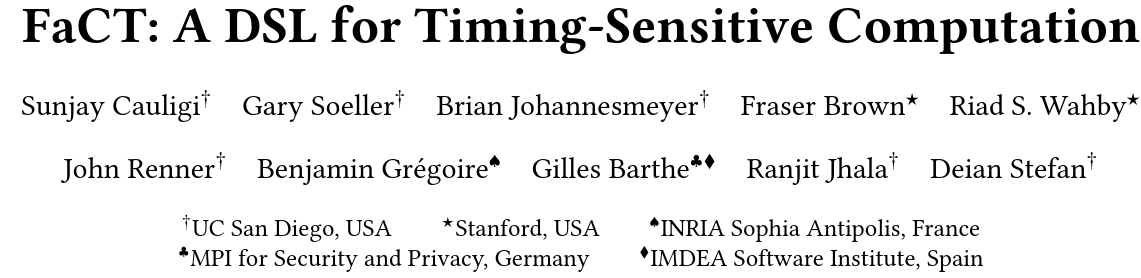
\includegraphics[width=0.8\textwidth]{../betterpl/fact-title}
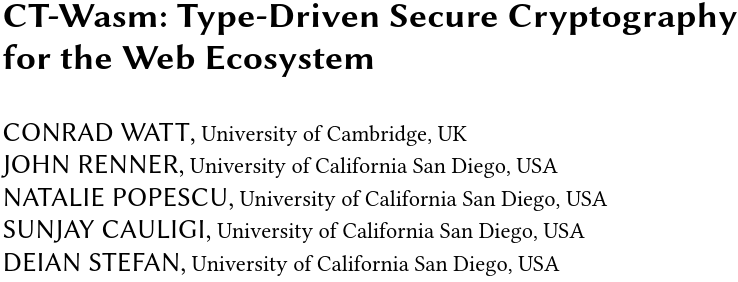
\includegraphics[width=0.8\textwidth]{../betterpl/ct-wasm-title}
\begin{itemize}
\item FaCT, PLDI 2019; CT-Wasm: POPL 2019
\end{itemize}
\end{frame}

\begin{frame}{constant-time programming languages}
    \begin{itemize}
    \item active research area, no consensus on what works best
    \vspace{.5cm}
    \item common approach: separate type for \textbf{secret} data
    \item compiler or language virtual machine disallows variable-time operations using secret data
    \item no secret-based array lookup (cache timing varies)
        \begin{itemize}
        \item e.g. array[secret\_value] $\rightarrow$ compile error (type mismatch)
        \end{itemize}
    \item no secret-based integer division (usually variable speed instruction)
    \item \ldots
    \vspace{.5cm}
    \item explicit operations for any secret-to-non-secret conversions
    \end{itemize}
\end{frame}


\section{backup slides}
\begin{frame}{backup slides}
\end{frame}
\subsubsection{example Linux concurrency UAF}
\begin{frame}{example: concurreny UAF bug}
\begin{tikzpicture}
\node (fig) {
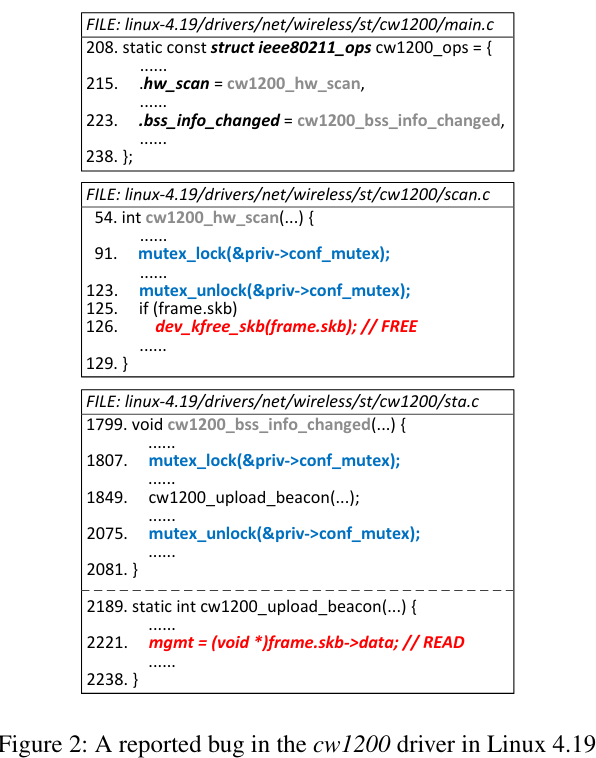
\includegraphics[height=0.9\textheight]{../betterpl/linux-conc-uaf-fig}
};
\node[anchor=north west,font=\small,align=left] at (fig.north east) {
Figure from Bai, Lawall, Chen and Mu \\ (Usenix ATC'19) \\
{\scriptsize ``Effective Static Analysis of Concurrency} \\ {\scriptsize Use-After-Free Bugs in Linux drivers''} \\
~ \\
bug in a wireless networking driver
};
\end{tikzpicture}
\end{frame}


\end{document}
